\documentclass[12pt,compress,ngerman,utf8,t]{beamer}
\usepackage[ngerman]{babel}
\usepackage{calc}
\usepackage{ragged2e,wasysym,multicol,mathtools}
\usepackage[protrusion=true,expansion=true]{microtype}
\usepackage{booktabs}
\hypersetup{colorlinks=true}

\graphicspath{{images/}}

\title{\large Wie ein seltsamer Trick der Chaostheorie die Raumfahrt revolutioniert}
\author[Ingo Blechschmidt]{\textcolor{white}{Ingo Blechschmidt \\ mit Dank an Sven Prüfer und Matthias Hutzler}}
\date[2017-01-04]{\vspace*{-5em}\ \\\textcolor{white}{\scriptsize Institut für Mathematik \\ Universität Augsburg \\ 4. Januar 2017 \\}}

%\usetheme{Warsaw}
\useinnertheme[shadow=true]{rounded}
\useoutertheme{split}
\usecolortheme{orchid}
\usecolortheme{whale}
\setbeamerfont{block title}{size={}}

\useinnertheme{rectangles}

\usecolortheme{seahorse}
\definecolor{mypurple}{RGB}{150,0,255}
\setbeamercolor{structure}{fg=mypurple}
\definecolor{myred}{RGB}{150,0,0}
\setbeamercolor*{title}{bg=myred,fg=white}
\setbeamercolor*{titlelike}{bg=myred,fg=white}

\usefonttheme{serif}
\usepackage[T1]{fontenc}
\usepackage{libertine}

\renewcommand{\_}{\mathpunct{.}\,}
\newcommand{\BB}{\mathbb{B}}
\newcommand{\M}{\mathcal{M}}
\newcommand{\R}{\mathrm{R}}
\newcommand{\NN}{\mathbb{N}}
\newcommand{\RR}{\mathbb{R}}

\newcommand{\imgslide}[1]{{\usebackgroundtemplate{\parbox[c][\paperheight][c]{\paperwidth}{\centering\includegraphics[width=\paperwidth]{#1}}}\begin{frame}[plain]\end{frame}}}

\setbeamertemplate{navigation symbols}{}

\setbeamertemplate{title page}[default][colsep=-1bp,rounded=false,shadow=false]
\setbeamertemplate{frametitle}[default][colsep=-2bp,rounded=false,shadow=false,center]

\newcommand{\hil}[1]{{\usebeamercolor[fg]{item}{\textbf{#1}}}}
\setbeamertemplate{frametitle}{%
  \vskip1em%
  \leavevmode%
  \begin{beamercolorbox}[dp=1ex,center]{}%
      \usebeamercolor[fg]{item}{\textbf{\textsf{\Large \insertframetitle}}}
  \end{beamercolorbox}%
}

\setbeamertemplate{footline}{%
  \leavevmode%
  \hfill%
  \begin{beamercolorbox}[ht=2.25ex,dp=1ex,right]{}%
    \usebeamerfont{date in head/foot}
    \insertframenumber\,/\,\inserttotalframenumber\hspace*{1ex}
  \end{beamercolorbox}%
  \vskip0pt%
}

\newcommand{\backupstart}{
  \newcounter{framenumberpreappendix}
  \setcounter{framenumberpreappendix}{\value{framenumber}}
}
\newcommand{\backupend}{
  \addtocounter{framenumberpreappendix}{-\value{framenumber}}
  \addtocounter{framenumber}{\value{framenumberpreappendix}}
}

\setbeameroption{show notes}
\setbeamertemplate{note page}[plain]

\begin{document}

% http://www.ufointernationalproject.com/wp-content/uploads/2015/11/a23.jpg
{\usebackgroundtemplate{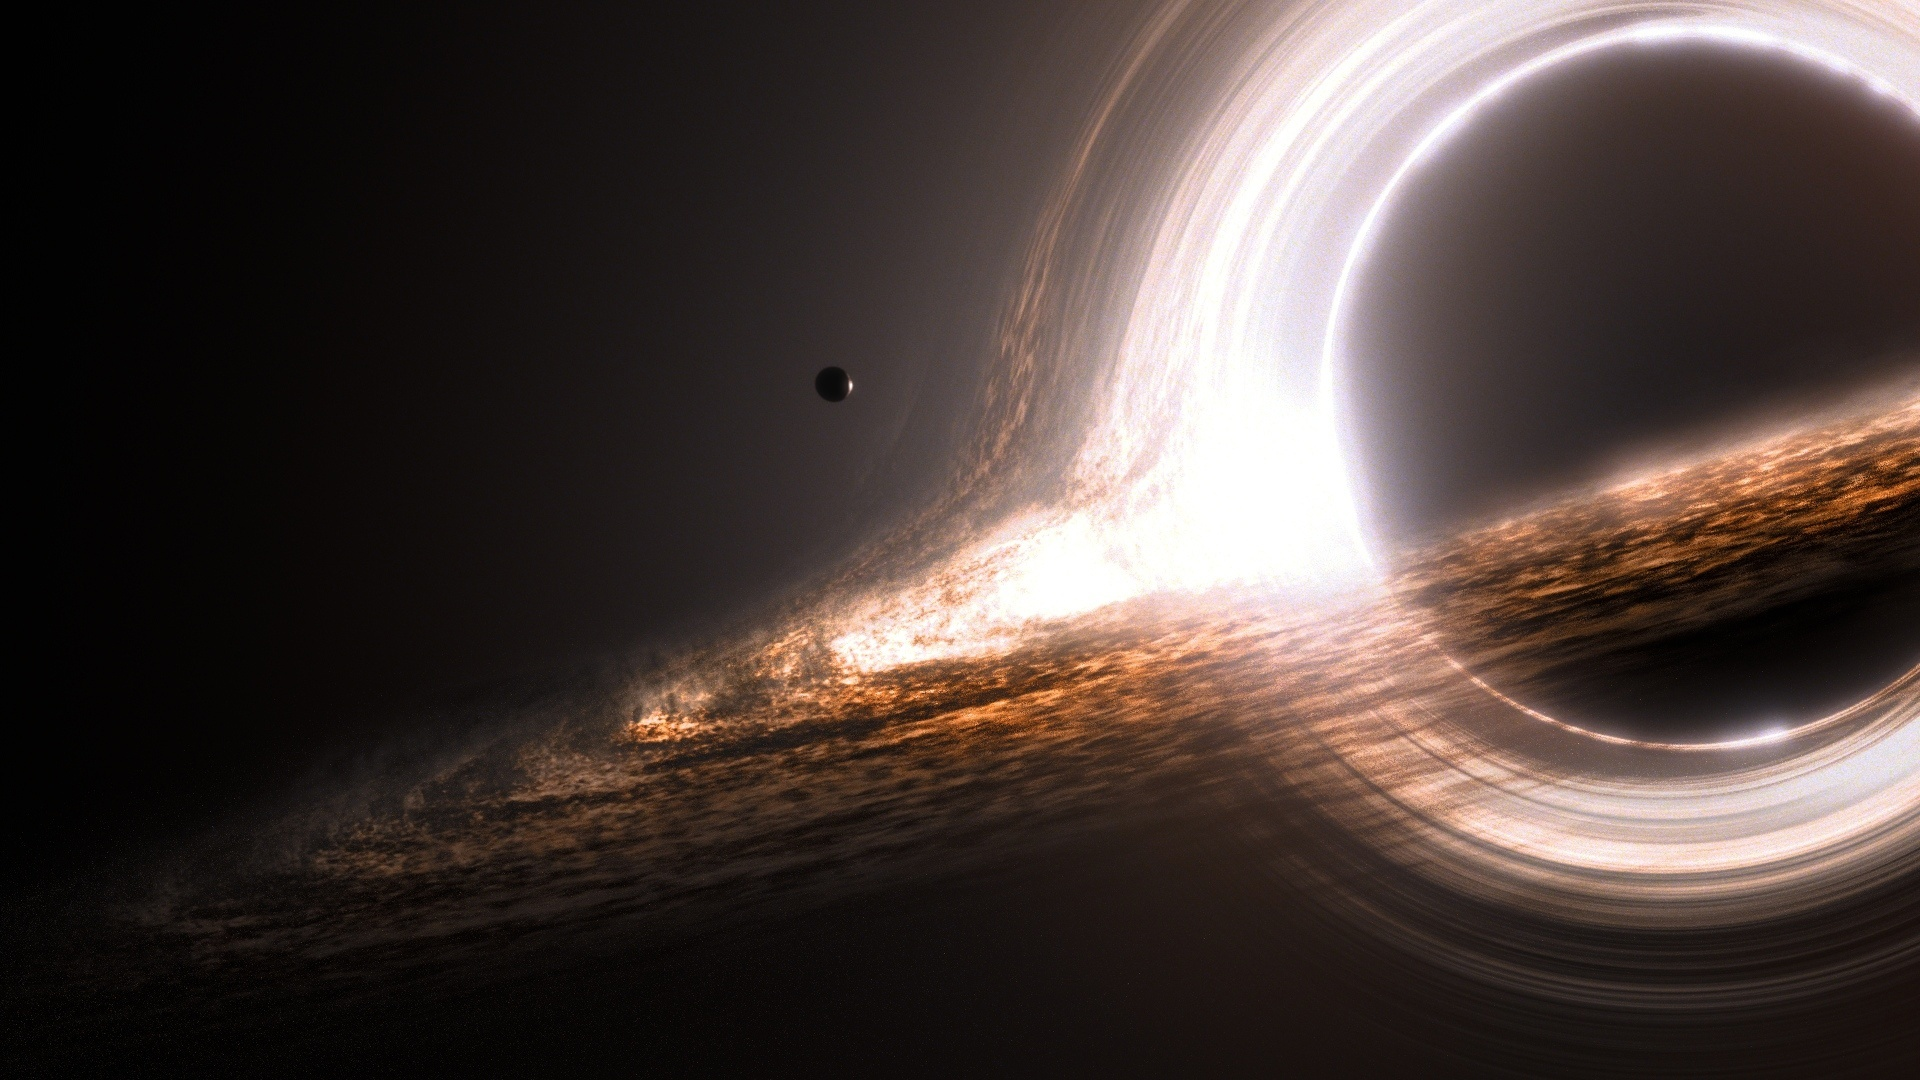
\includegraphics[height=\paperheight]{images/interstellar}}
\frame{\vspace*{9em}\titlepage}}
\imgslide{clips/01-wormholes}
\frame{\tableofcontents}


\section[Crashkurs in Orbitalmechanik]{Ein Crashkurs in Orbitalmechanik}

{\usebackgroundtemplate{\begin{minipage}{\paperwidth}\vspace*{6.5cm}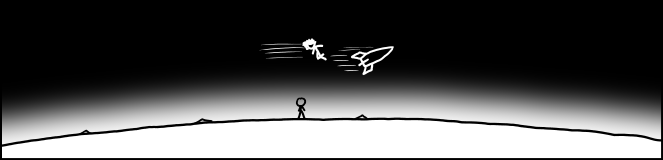
\includegraphics[width=\paperwidth]{images/orbit-wide}\end{minipage}}
\begin{frame}
  \centering
  \bigskip\bigskip

  \Huge \hil{Teil I}

  \bigskip
  \Large\textbf{Ein Crashkurs in Orbitalmechanik}
  \par
\end{frame}}

{\usebackgroundtemplate{\begin{minipage}{\paperwidth}\hfill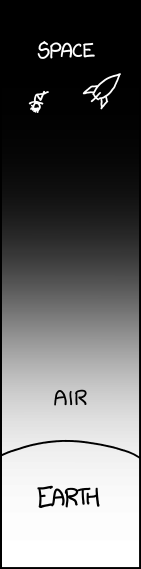
\includegraphics[height=\paperheight]{images/orbit-tall}\end{minipage}}
\begin{frame}{Grundlagen}
  \begin{itemize}
    \item Es ist leicht, ins Weltall zu kommen. \\ Schwer ist es, dort zu bleiben.
    \item Die Erdbeschleunigung auf Höhe der ISS ist \\ immer noch $\approx 8{,}7 \,\mathrm{m}/\mathrm{s}^2$.
    % Mention: no friction.
  \end{itemize}
\end{frame}}


\subsection{Grundlagen}

\begin{frame}{Grundlagen}
  \begin{itemize}
    \item<1-> Es ist leicht, ins Weltall zu kommen. \\ Schwer ist es, dort zu bleiben.
    \item<3-> Geschwindigkeit ist wichtig.
    \item<4-> Im \hil{Einkörperproblem} gibt es nur drei Arten von Orbiten: elliptische, parabolische und hyperbolische.
    \item<5-> Sei dir deiner Annahmen bewusst:
    \begin{enumerate}
      \item Ist die Erde eine perfekte Kugel?
      \item Hat sie Atmosphäre?
      \item Dreht sie sich um sich selbst?
    \end{enumerate}
    % instantaneous impulses?
  \end{itemize}

  \only<1>{
    \centering
    % https://upload.wikimedia.org/wikipedia/commons/thumb/7/73/Newton_Cannon.svg/240px-Newton_Cannon.svg.png
    \vspace*{-7em}
    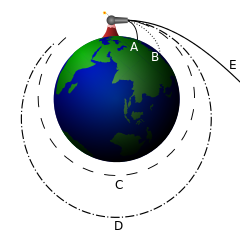
\includegraphics[width=0.4\textwidth]{images/newton-cannon}

    $F_{\text{centripetal}} = F_{\text{gravitation}}
    \leadsto v_1 = \sqrt{GM/r}$

    $E_{\text{kinetic}} = E_{\text{gravitation}}
    \leadsto v_2 = \sqrt{2} \, v_1$
    \par
  }

  \only<2>{
    \centering
    \vspace*{-4em}
    \begin{tabular}{ll}
      \toprule
      Himmelskörper & zweite Fluchtgeschwindigkeit \\\midrule
      Erde & $11{,}2 \,\mathrm{km}/\mathrm{s} \approx 40\,000 \,\mathrm{km}/\mathrm{h}$ \\
      Mond  & $2{,}4  \,\mathrm{km}/\mathrm{s}$ \\
      Sonne & $618  \,\mathrm{km}/\mathrm{s}$ \\
      Milchstraße & $\approx 550 \,\mathrm{km}/\mathrm{s}$ \\
      \bottomrule
    \end{tabular}
    \par
  }
\end{frame}


\subsection{Orbitwechsel}

\begin{frame}{Orbitwechsel}
  \begin{center}
    \hil{``Live-Demo''}
  \end{center}

  \begin{itemize}
    \item Änderung der Phase

    % Winkel ändern:
    % Speed away from the central body.
    % Necessary Δv depends on eccentricity.
    % If eccentricity is zero, need to Δv.

    \item Änderung der Exzentrizität
    % Accelerate in tangential direction

    \item Änderung des Radius
    % Hohmann transfer

    \item Änderung der Ebene
    % Easy, just accelerate normal to the plane.
  \end{itemize}
\end{frame}

\imgslide{clips/02-chinese-space-station}


\subsection[Raketengleichung]{Die Tyrannei der Raketengleichung}

\begin{frame}{Die Tyrannei der Raketengleichung}
  \centering
  % http://tsiolkovsky.org/wp-content/uploads/2015/02/icon_en.png
  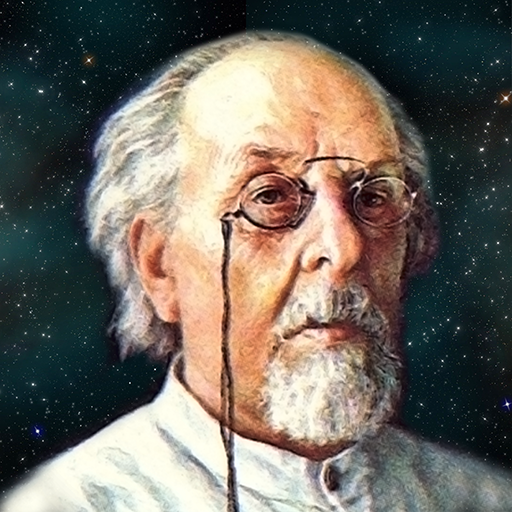
\includegraphics[width=0.4\textwidth]{images/tsiolkovsky} \\
  {\scriptsize Konstantin Tsiolkovsky (* 1857, † 1935)\par}
  \bigskip

  \scalebox{2}{$m_\text{total} = m_\text{payload} \cdot e^{\Delta v / v_\text{eff.\@ exhaust}}$}
  \par
\end{frame}

% Weltall ist nah.
% Extrem wichtig: (Ort,Geschwindigkeit) des Ziels
% Erste Fluchtgeschwindigkeit
% Filmausschnitt Bruce Willis
% Filmausschnitt Gravity?
% Arten von Trajektorien (stets Ellipsen, Parabeln oder Hyperbeln)
% Tyrannei der Raketengleichung
% Orbitwechsel
% Gravity assist


\section[Chaostheorie]{Ein seltsamer Trick der Chaostheorie}

{\usebackgroundtemplate{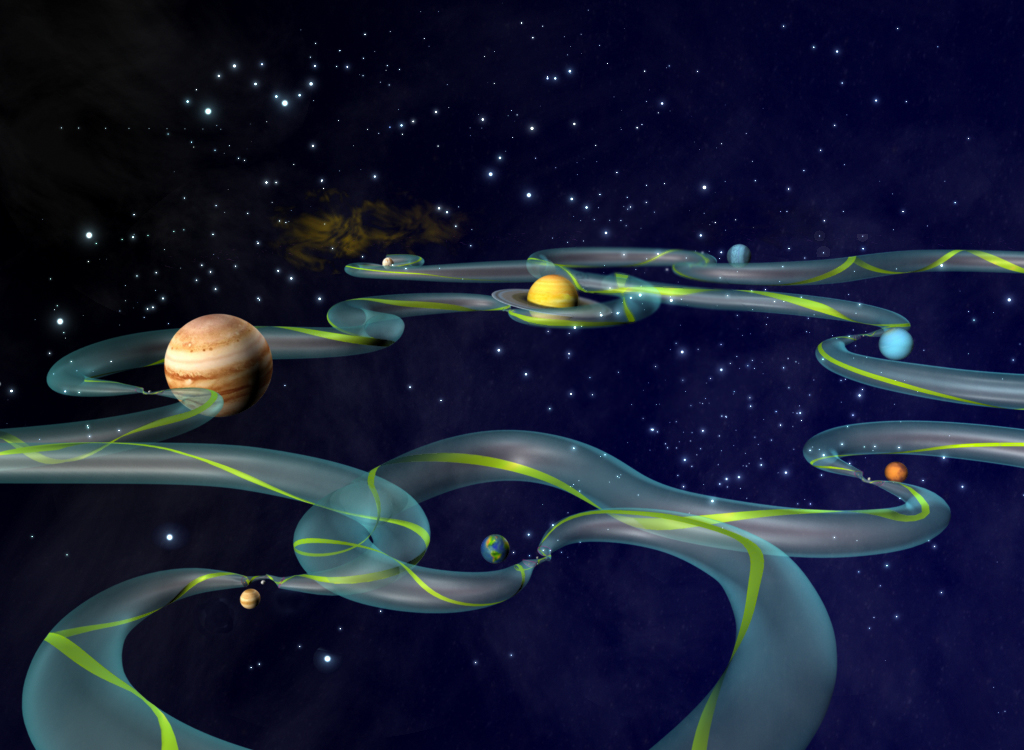
\includegraphics[height=\paperheight]{images/Interplanetary_Superhighway}}
\begin{frame}
  \centering
  \bigskip\bigskip

  \Huge \hil{Teil II}

  \bigskip
  \Large\textcolor{white}{\textbf{Ein seltsamer Trick der Chaostheorie}}
  \par
\end{frame}}


\subsection{Lagrange-Punkte}

\begin{frame}{Lagrange-Punkte}
  \centering
  \only<1>{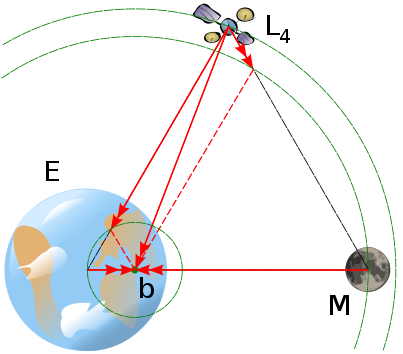
\includegraphics[width=0.7\textwidth]{lagrange}}
  \only<2>{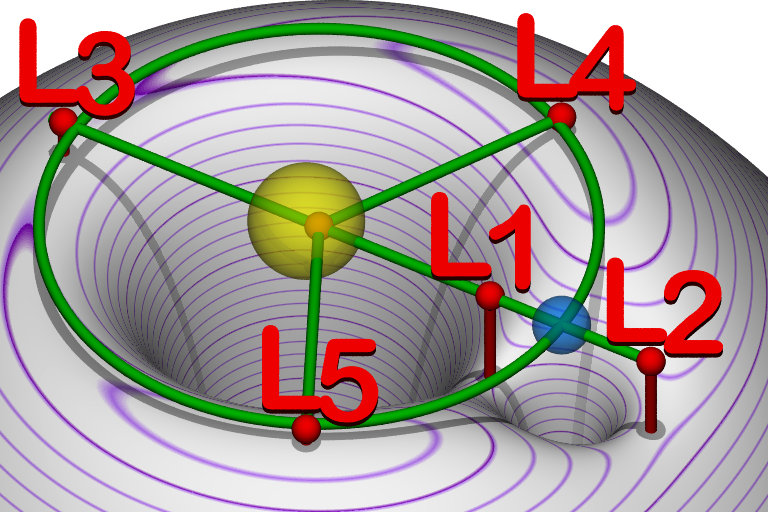
\includegraphics[width=0.7\textwidth]{lagrange2}}
  \par
\end{frame}


\subsection{Weak stability boundaries}

\begin{frame}{Weak stability boundaries}
  \centering
  \only<1>{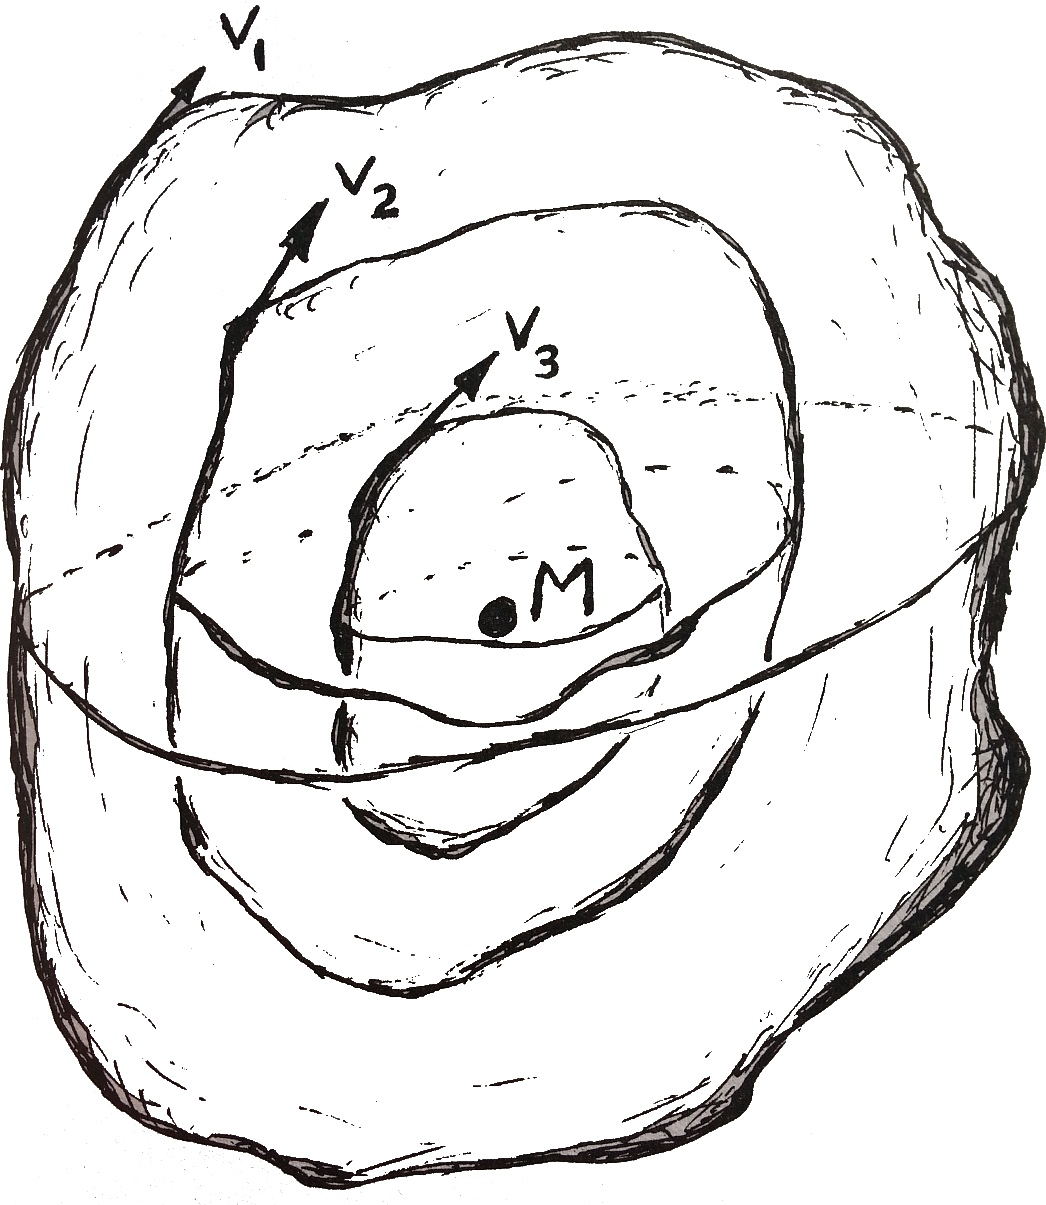
\includegraphics[width=0.6\textwidth]{weak-stability-boundaries}}
  \only<2>{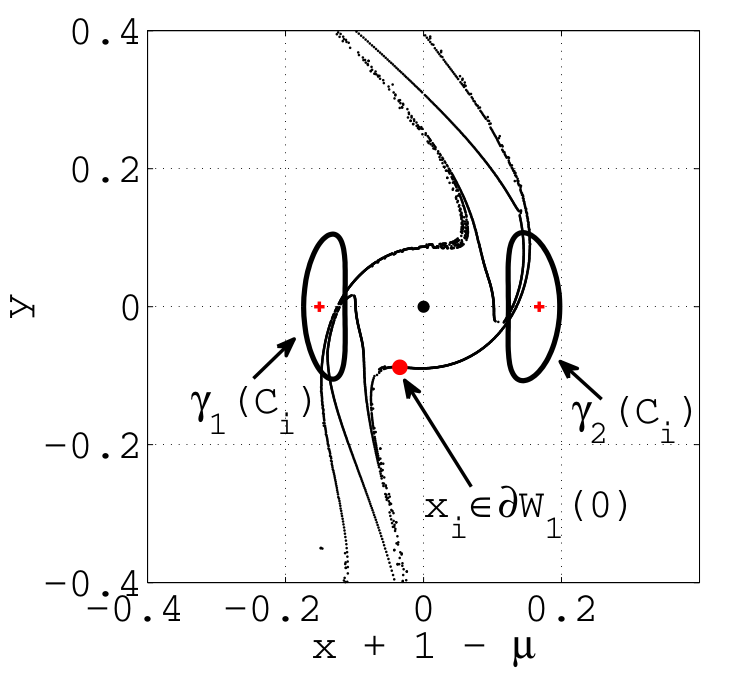
\includegraphics[width=0.7\textwidth]{weak-stability-boundary-plot}}
  \par
\end{frame}

\imgslide{clips/03-supercomputer-1}


\subsection[Hiten]{Die Rettung der Hiten}

\begin{frame}{Die Rettung der Hiten}
  \centering
  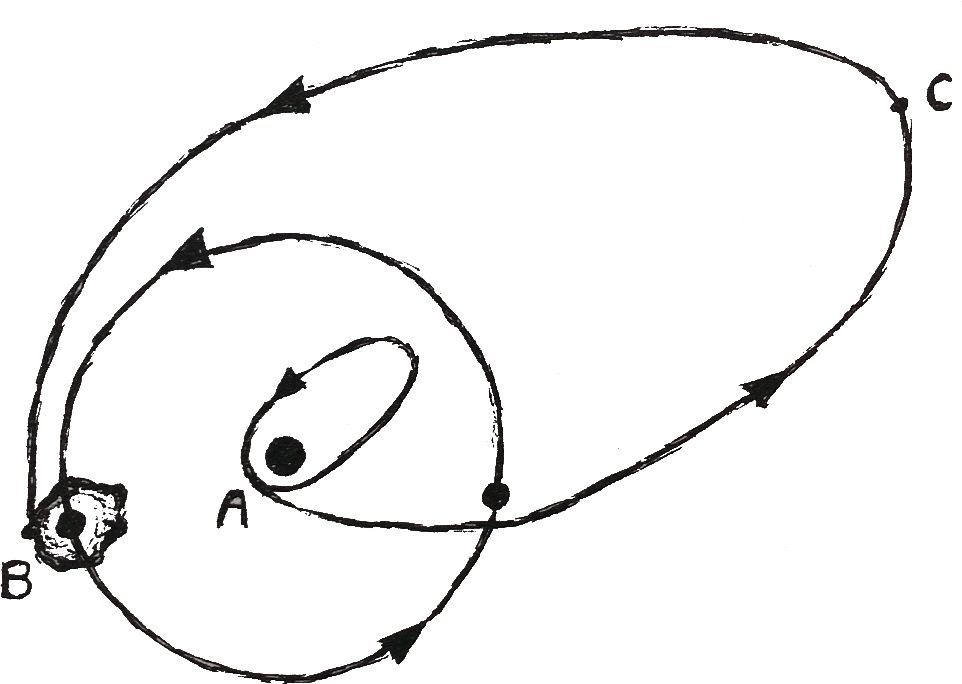
\includegraphics[width=0.7\textwidth]{hiten-trajectory}
  \par
\end{frame}


\subsection{In der Natur}

\begin{frame}{In der Natur}
  \centering
  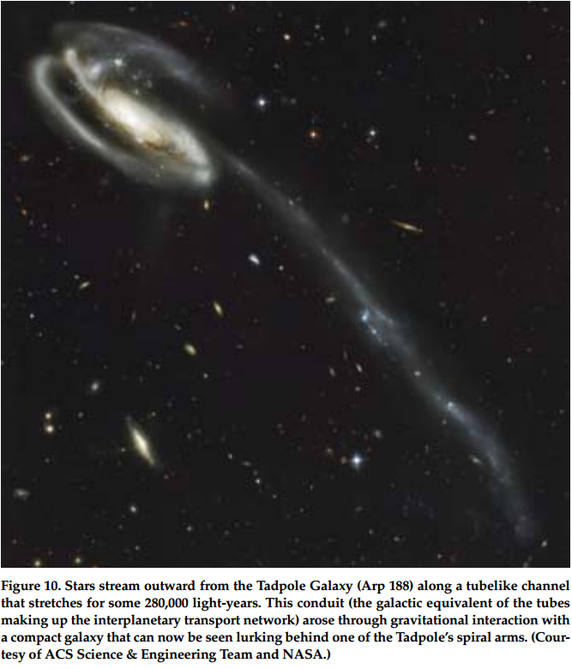
\includegraphics[width=0.6\textwidth]{intergalactic-transport-network}
  \par
\end{frame}

% https://upload.wikimedia.org/wikipedia/commons/thumb/7/78/L4_diagram.svg/403px-L4_diagram.svg.png
% https://upload.wikimedia.org/wikipedia/commons/5/5f/Lagrangian_points_equipotential.jpg

% Zunächst: Orbiten komplizierter!
% Probleme mit konventionellem Ansatz (auch Neustartprobleme)
% Ziel: ballistisches Einfangen
% Lagrange-Punkte (Krassheit der Punkte nicht vergessen)
% dazu mitrotierendes Bezugssystem, Zentrifugalkraft, Corioliskraft
% WSM
% Wie man sie findet
% Hiten
% In der Natur

% Wurmlochnostalgie nicht vergessen!
% Krasse Rundtourtrajektorien nicht vergessen!
% Szene aus The Martian nicht vergessen!
% Szene aus Gravity nicht vergessen!
% Swing-by-Manöveur nicht vergessen!
% Hohmann-Transfer nicht vergessen!
% Krasse Stärke der Gravitation beiläufig erwähnen.

\end{document}
